\documentclass{article}

\usepackage{amsmath}
\usepackage{graphicx}
\usepackage{xcolor}
\usepackage[export]{adjustbox}
\RequirePackage[margin=1in]{geometry}

\newcommand\todo[1]{\textcolor{red}{TODO: #1}}

\newcommand\animation[1]{\textcolor{blue}{ANIMATION: #1}}

\begin{document}
	
\title{Hillshade Video Script}
\author{Nathan Stouffer}
\date{}
\maketitle

\section{Intro}

\subsection{Motivation (about 50s)}

When you look at the map shown below, I bet much of the terrain's shape is evident to you.
I'd guess that know this spot to be pretty flat and this other area to be relatively steep.
Possibly you can pick out a gully right here and a ridgeline over there.
Or maybe you've noticed that this face is pretty rugged while this slope is smooth.

Regardless of what individual features you've noticed, I'm certain you have some notion of what this terrain looks like even though all you can see is a greyscale image.

This map is intentionally set up so that your brain can intuit the shape of the terrain.
Computers do much of this work today, but cartographers have been using this technique for hundreds of years.
And many other applications use similar strategies to help convey geometric information.

The topic I'd like to discuss today is a lighting technique called hillshade.
We're going to see why it's an effective method of illumination and walk through the math that powers it.

\begin{center}
	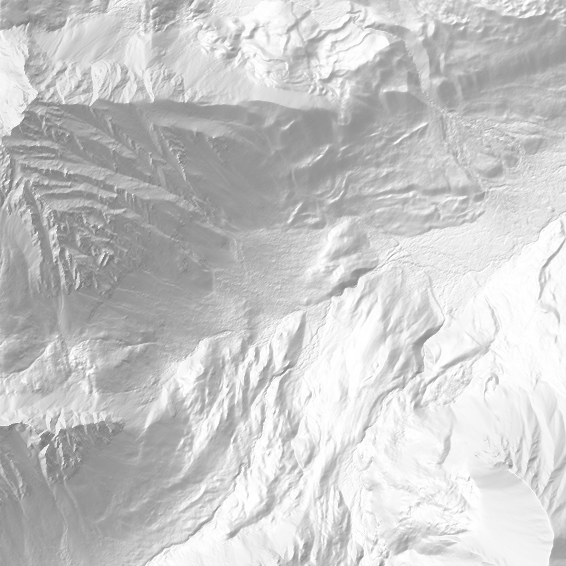
\includegraphics[width=0.5\textwidth,frame]{assets/hillshade-example.png}
\end{center}

\subsection{Directional Lighting (about 2m 20s)}

The particular topic we'll be discussing is hillshade, but it's worth mentioning that hillshade is a very specific example of something called a directional light.
Directional lights are used all over computer graphics and are themselves just one option for how you might want to light a scene.
What I find so intriguing about directional lights is that they give you a lot of bang for your buck.
You get a lot of realism for the amount of effort that you need to expend.

\animation{Fade in a graph similar to the below image.}

\begin{center}
	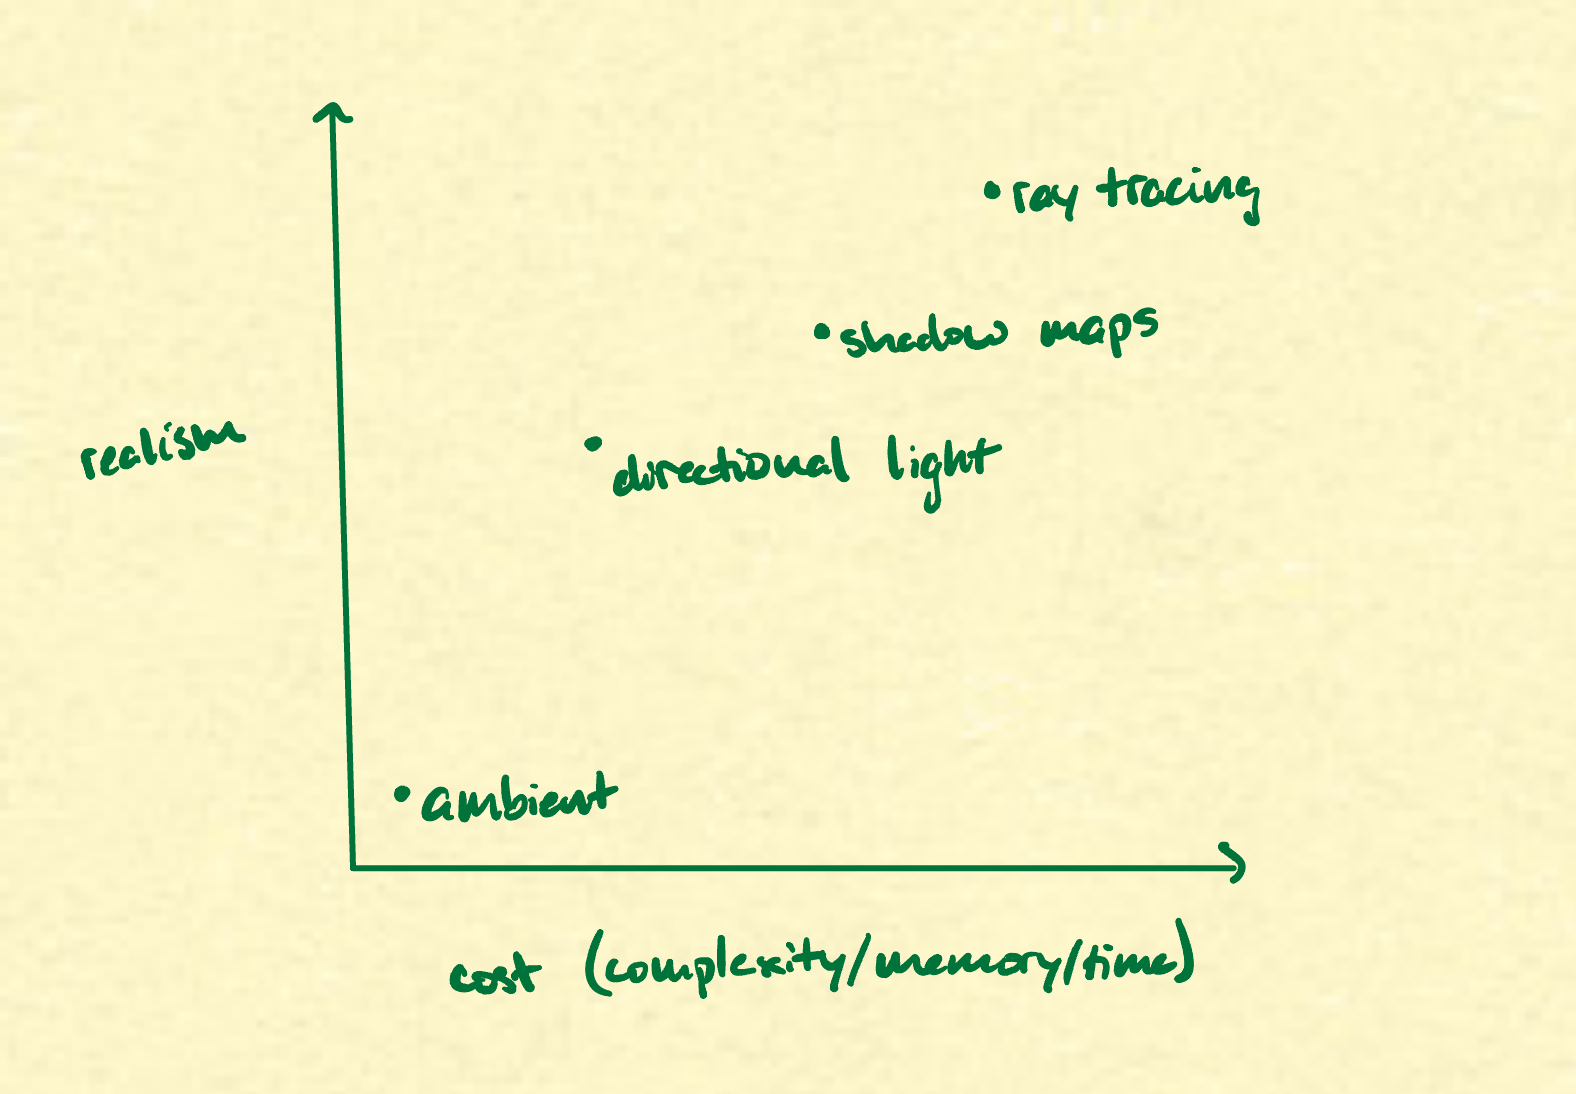
\includegraphics[width=0.65\textwidth,frame]{assets/realism.jpg}
\end{center}

If you were to represent different lighting techniques as points in the plane where the y-axis represents some notion of realism (how realistic a scene looks) and the x-axis represents some notion of cost (maybe in terms of complexity/memory/computation time).
Then on that graph, directional lights would exist at a sweet spot where they are unreasonably effective -- they don't cost that much but they provide a healthy amount of realism.

Let's get into the details of what a directional light is.
A directional light is a pseudo-realistic model of how light behaves.
In the interest of simplicity, directional lights take a few shortcuts:

\begin{enumerate}

\item First, they ignore obstructions.
What this means is that we won't compute true shadows -- just whether or not an object is looking at the light source.
This is the piece of directional lights that I find to be the most interesting: even when ignoring obstructions, directional lights give enough hints of realism to trick your brain into thinking objects are 3D.

\animation{Demonstrate a simple example of shadows in 2D}.
	
\item Second, directional lights assume the light source to be extremely far away.
This assumption means that every point in the scene has light coming from the same direction $l$ -- giving the technique its name.

To make the math a little simpler, I am actually going to use the negative of the light direction.
This makes $l$ the vector that points directly \textit{towards} the light source.

\end{enumerate}

The direction that the terrain faces is encoded in something called a surface normal.
If we zoom in on a very small portion of the terrain, then it can be reasonably approximated as a small plane.
The outward pointing vector that is orthogonal to the approximating plane is called a surface normal.

\animation{Show a rotating plane with a surface normal that is lit according to hillshade.}

The effect we are looking for should behave like this:
If the terrain generally points in the same direction as the light, we want the terrain to be pretty bright.
If the light direction kind of glances off the terrain, we want the terrain to be a tone of grey.
And if the terrain generally faces away from the light direction, we want the terrain to be dark.

\section{Hillshading}

At this point, we've covered what the effect should do, but how can we accomplish it?
What are the nuts and bolts that turn this loose discussion into a sequence of mathematical operations?

\subsection{Cosine (about 1m 50s)}

We can start by being more precise about describing how the light strength should vary.
Let's represent a small area of the terrain as a rotated square.
When $n$ and $l$ point in the exact same direction, we want to light at full strength.
And we know we want to decrease the strength of the light as the angle between $n$ and $l$ increases.
To root some of our model in reality, we will vary the intensity of the shading based on how much light is blocked by the rotated square - ie the area of its shadow.

I won't prove this for you, but it so happens that (with a directional light) the signed area of a rotated square's shadow is $A * \cos \theta$ where $A$ is the area of the square, $\theta$ is the angle between $l$ and $n$, and the sign encodes whether or not the square faces the light source (positive means facing the light source and negative means facing away).
If an un-rotated square gets the full light strength of $1$, then this fact implies that a rotated square gets strength $S = 1 * \cos \theta = \cos \theta$.

You might notice that $\cos \theta$ can be negative.
What are we to do with a negative light strength?
Well, it depends on the application.
Some directional light models ignore negative light strengths.
Hillshade takes a slightly different approach.
Our goal is to effectively illuminate a map so that the reader can see terrain features.
When we ignore negative light strength, we effectively remove shading on all terrain that faces away from the light source.
Instead, it is more effective to remap the range of cosine to the interval $[0, 1]$.
This can be done by first adding 1 to the result and then dividing by 2.
 
\animation{Transform the range of cosine via $\dfrac{1}{2}(1 + \cos \theta)$}

\begin{center}
	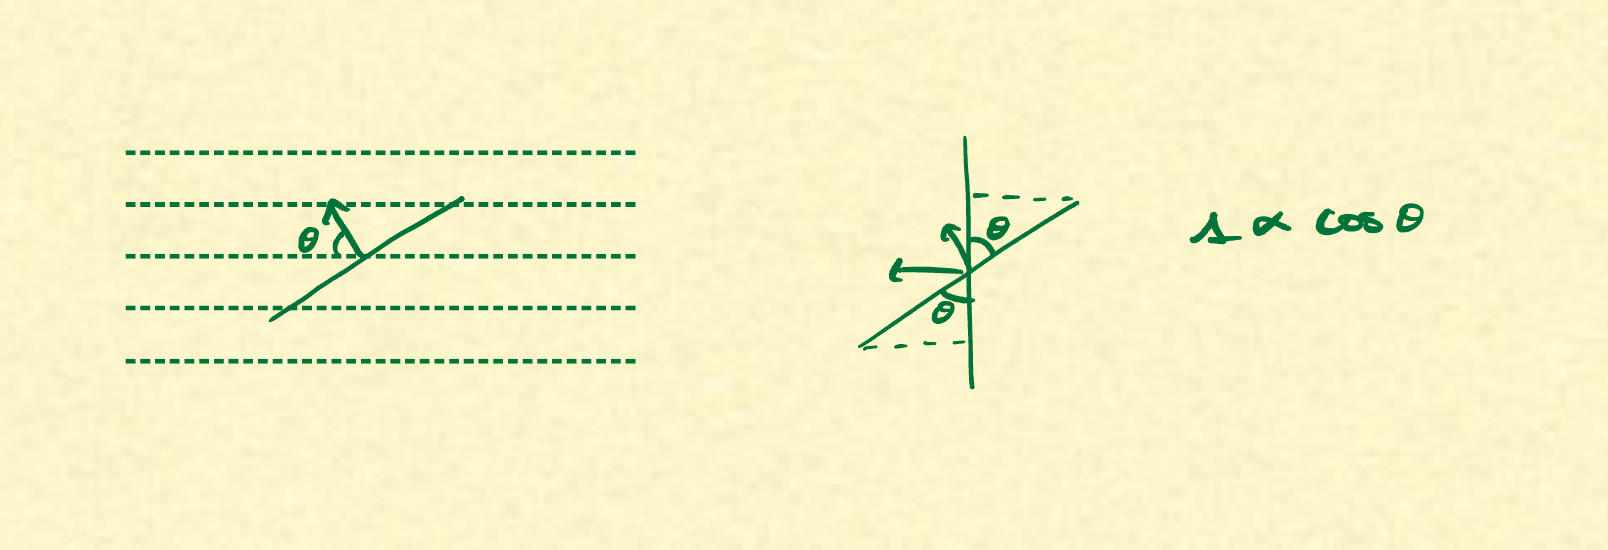
\includegraphics[width=0.75\textwidth,frame]{assets/cosine.jpg}
\end{center}

\subsection{Law of Cosines (about 2m)}

We now know that we want to vary the strength of our lighting according to $\cos \theta$.
But that doesn't really help us much because we don't know what $\theta$ is -- all we know are the vectors $l$ and $n$.
At the end of the day, those are just lists of numbers.
What is the link between these two vectors and cosine?

If we were solving this on our own, we would need to start experimenting and see if inspiration strikes.
It might take a lot of tries and result in quite a few dead ends.
It's one of those things where experience is the best teacher.

... But if I were to offer one piece of advice, I would say it's often worth constructing a triangle.
Maybe it's the type of problems that I interact with, but I find triangles to be an extremely effective tool.
In this case, we are going to draw the third leg of our triangle here and use the Law of Cosines.

\begin{center}
	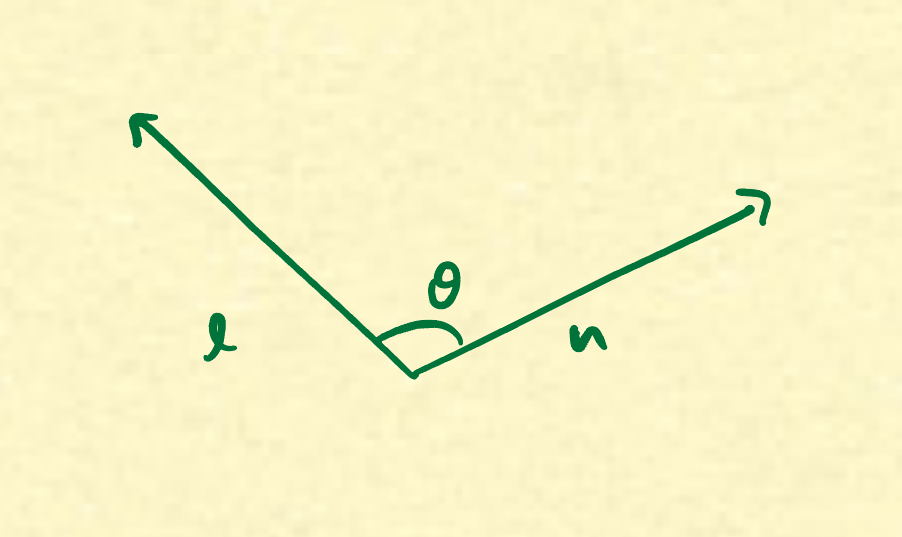
\includegraphics[width=0.3\textwidth,frame]{assets/ln.jpg}
	\hspace{0.2\textwidth}
	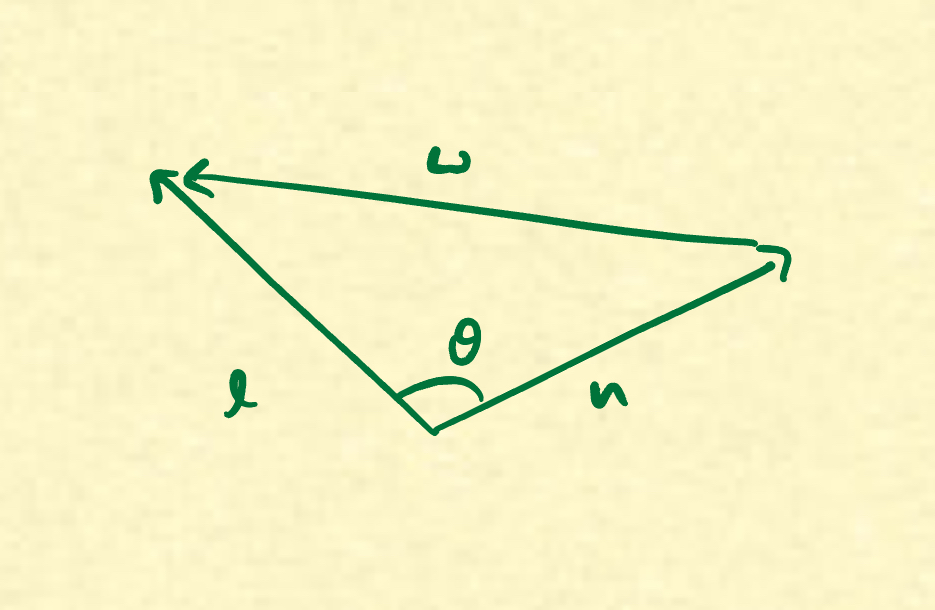
\includegraphics[width=0.2735\textwidth,frame]{assets/lnw.jpg}
\end{center}

The full Law of Cosines says that for any triangle with sides/angle labeled like so, we have the following equality: $c^2 = a^2 + b^2 - 2ab \cos C$.
In our case, $a = |l|$, $b = |n|$, and $C = \theta$.
The third side of our triangle is the difference between $l$ and $n$ so its length is magnitude of that difference.

\begin{align*}
|l-n|^2 = |l|^2 + |n|^2 - 2 |l| |n| \cos \theta & \quad \text{substitute from generalized LoC} \\
|l-n|^2 = 2 - 2 \cos \theta & \quad \text{didn't discuss this earlier, but } |l| = |n| = 1 \\
1 - \dfrac{1}{2}|l-n|^2 = \cos \theta & \quad \text{simplifying}
\end{align*}

I didn't mention this earlier, but by convention, $l$ and $n$ are unit vectors -- meaning their magnitude is 1.
If we use that fact and then simplify, we can compute $\cos \theta$ from values that we already know: the vectors $l$ and $n$.

If you are familiar with the dot product, you know that this can be simplified further.
But in the interest of accessibility, I'm going to leave it here because we have what we need.

\section{Final product (about 30s)}

And that pretty much wraps it up.
From our shadow area discussion, we know the strength of our light is $\dfrac{1}{2}(1 + \cos \theta)$ and we just figured out how to compute $\cos \theta$ in terms of the two things we know: the vectors $l$ and $n$.
Computing that value for each pixel is all it takes to produce the beautiful images shown below.
It never ceases to amaze me how such simple a computation can produce stunning and realistic results.

\animation{Show a few examples.}

\section{Endnotes}

I'd like to close the video by making a few comments.

\subsection{Modifications (about 25s)}

Hillshade isn't just one thing.
It's actually a term for a family of effects that can be applied to a map.
There are a lot of variations out there.
Different models might add ambient light, exaggerate the terrain, use multiple light sources, or play around with colored lights.
You now have the mathematical framework that sits behind all of them.

\todo{Possibly mention Eduard Imhof.}

\subsection{Pseudoscopic Illusion (about 30s)}

Most people have an easier time recognize terrain features when the light is placed in the top left of an image.
Because many maps use a north-up convention, hillshade is typically lit from the northwest.

However, this can sometimes backfire when a map with static hillshade is oriented with a south-up convention.
When that occurs, your brain might interpret everything backwards (ie valleys as ridges and ridges and valleys).
This is called a pseudoscopic illusion.

\animation{Show a south-up map light from the northwest and then fade in the same map (still south up) with a southeast (top left) light}.

\subsection{Simplicity (about 30s)}

For my final comment, I'd like revisit the simplicity of this effect -- I just can't get over it!
As we've discussed, the math is pretty simple yet the results are unreasonably effective.
But what's even crazier is the fact that all the maps you've seen in this video are 2-dimensional -- and I don't just mean that the screen you're viewing is 2-dimensional.
I mean that the actual model that I am rendering is 2D.

\animation{Pitch the camera}

Despite that, at least to me, hillshade vividly evokes the 3D nature of terrain.
I find that fascinating.

\animation{3D flythrough?}

\end{document}